\chapter{工程概况}
\section{供电方式}
在我国,用电负荷根据重要程度可分为一级负荷、二级负荷和三级负荷。其中一级负荷应由两路独立电源供电,当任何一路电源发生故障中断供电时,另一路应能保证继续供电。在城市轨道交通供电系统中,牵引用电负荷为一级负荷,而动力照明等用电负荷根据实际情况可分为一级、二级或三级负荷。城市轨道交通的外部电源供电方案应根据供电公司线网规划和城市电网的具体情况进行规划设计,而不应局限在某一条线路上。根据实际情况的不同,外部电源方案可分为集中供电方式、分散供电方式和混合供电方式。
\par 现我国大多数城市地铁多采用集中供电方式,而有轨电车一般采用分散供电方式或混合供电方式。\par
集中供电方式是指在线路的适当站位,根据总容量的要求设置主变电所,由发电厂或城市电网区域变电所以高压(常见的如110kV)向主变电所供电,经主变电所降压成中压(常见的如35kV或10kV)向各车站变电所供电,结合各车站变电所进线形成中压环网,再由环网供沿线设置的牵引变电所,并降压整流为直流电(如750V或1500V),从而对电动列车供电。另外,各车站机电设备用电需由降压变电所降压为AC380/220V。为了便于城市轨道交通供电系统的统一管理,城市轨道交通供电系统目前较多地采用集中供电方式。这种供电方式的中压网络电压等级的确定,需要考虑用电容量、供电距离、城市当地电网现状及发
展规划等因素。\par
分散供电方式是指不设置主变电所,而直接由城市电网区域变电所的35kV或10kV 中
压供电线路直接向城市轨道交通沿线设置的牵引变电所、降压变电所供电并形成环网。采用这种供电方式的前提是城市电网比较发达,并且在有关车站附近有符合可靠性要求的供电电
源,其中压网络的电压等级应与城市电网相一致。分散供电方式可设置电源开闭所,并可与
车站变电所合建。\par
混合供电方式,是以上两种方式的混合,即轨道交通线路的一部分采用集中供电方式,
另一部分采用分散供电方式,但一般以集中供电方式为主、分散供电方式作为补充。\par
集中式供电的优点:\newline
(1)可靠性高,便于集中统一调度和集中管理。\newline
(2)施工方便,维护容易,电缆敷设径路比较好走。\newline
(3)抑制谐波的效果较好。为减少谐波对电网的影响和危害,一是采用较高脉波(24脉波)整流机组,二是选用较高电压(110kV) 的电源,因为大容量、高电压电网的承受能力强,同时国标规定的谐波总畸变率和谐波电压含有率比小容量、低电压电网要低得多,而且也有利于今后集中采取高次谐波防治措施。\newline
(4)计费方便、简单。采用110kV电压集中供电方式,运行管理单位与电业部门的电度计费在主变电所设总计量就行,不必在各变电所分别计量。\par 
所以决定采用集中式供电方式
\section{供电电压方式}
集中供电方式:城市电网向城市轨道交通的专用主变电所供电,经降压并在沿线结合牵引变电所和降压变电所形成中压环网,向轨道交通各系统供电, 分散供电方式:不设主变电所,直接由城市电网区域变电所的中压输电线直接向轨道交通沿线设置的牵引变电所、降压变电所供电并形成环网。由于使用的是集中供电方式,所以使用三级式供电电压方式。在城市轨道交通沿线,根据用电容量和线路长短,建设专用的主变电所。主变电所进线电压一般为110kV,经降压后变成35kV或10kV,供给牵引变电所与降压变电所。主变电所应有两路独立的进线电源。集中式供电,有利于城市轨道交通供电形成独立体系,便于管理和运营。采用集中式供电的有上海、 广州、南京、香港、德黑兰地铁等。\par
% TODO: \usepackage{graphicx} required
\begin{figure}[h]
	\centering
	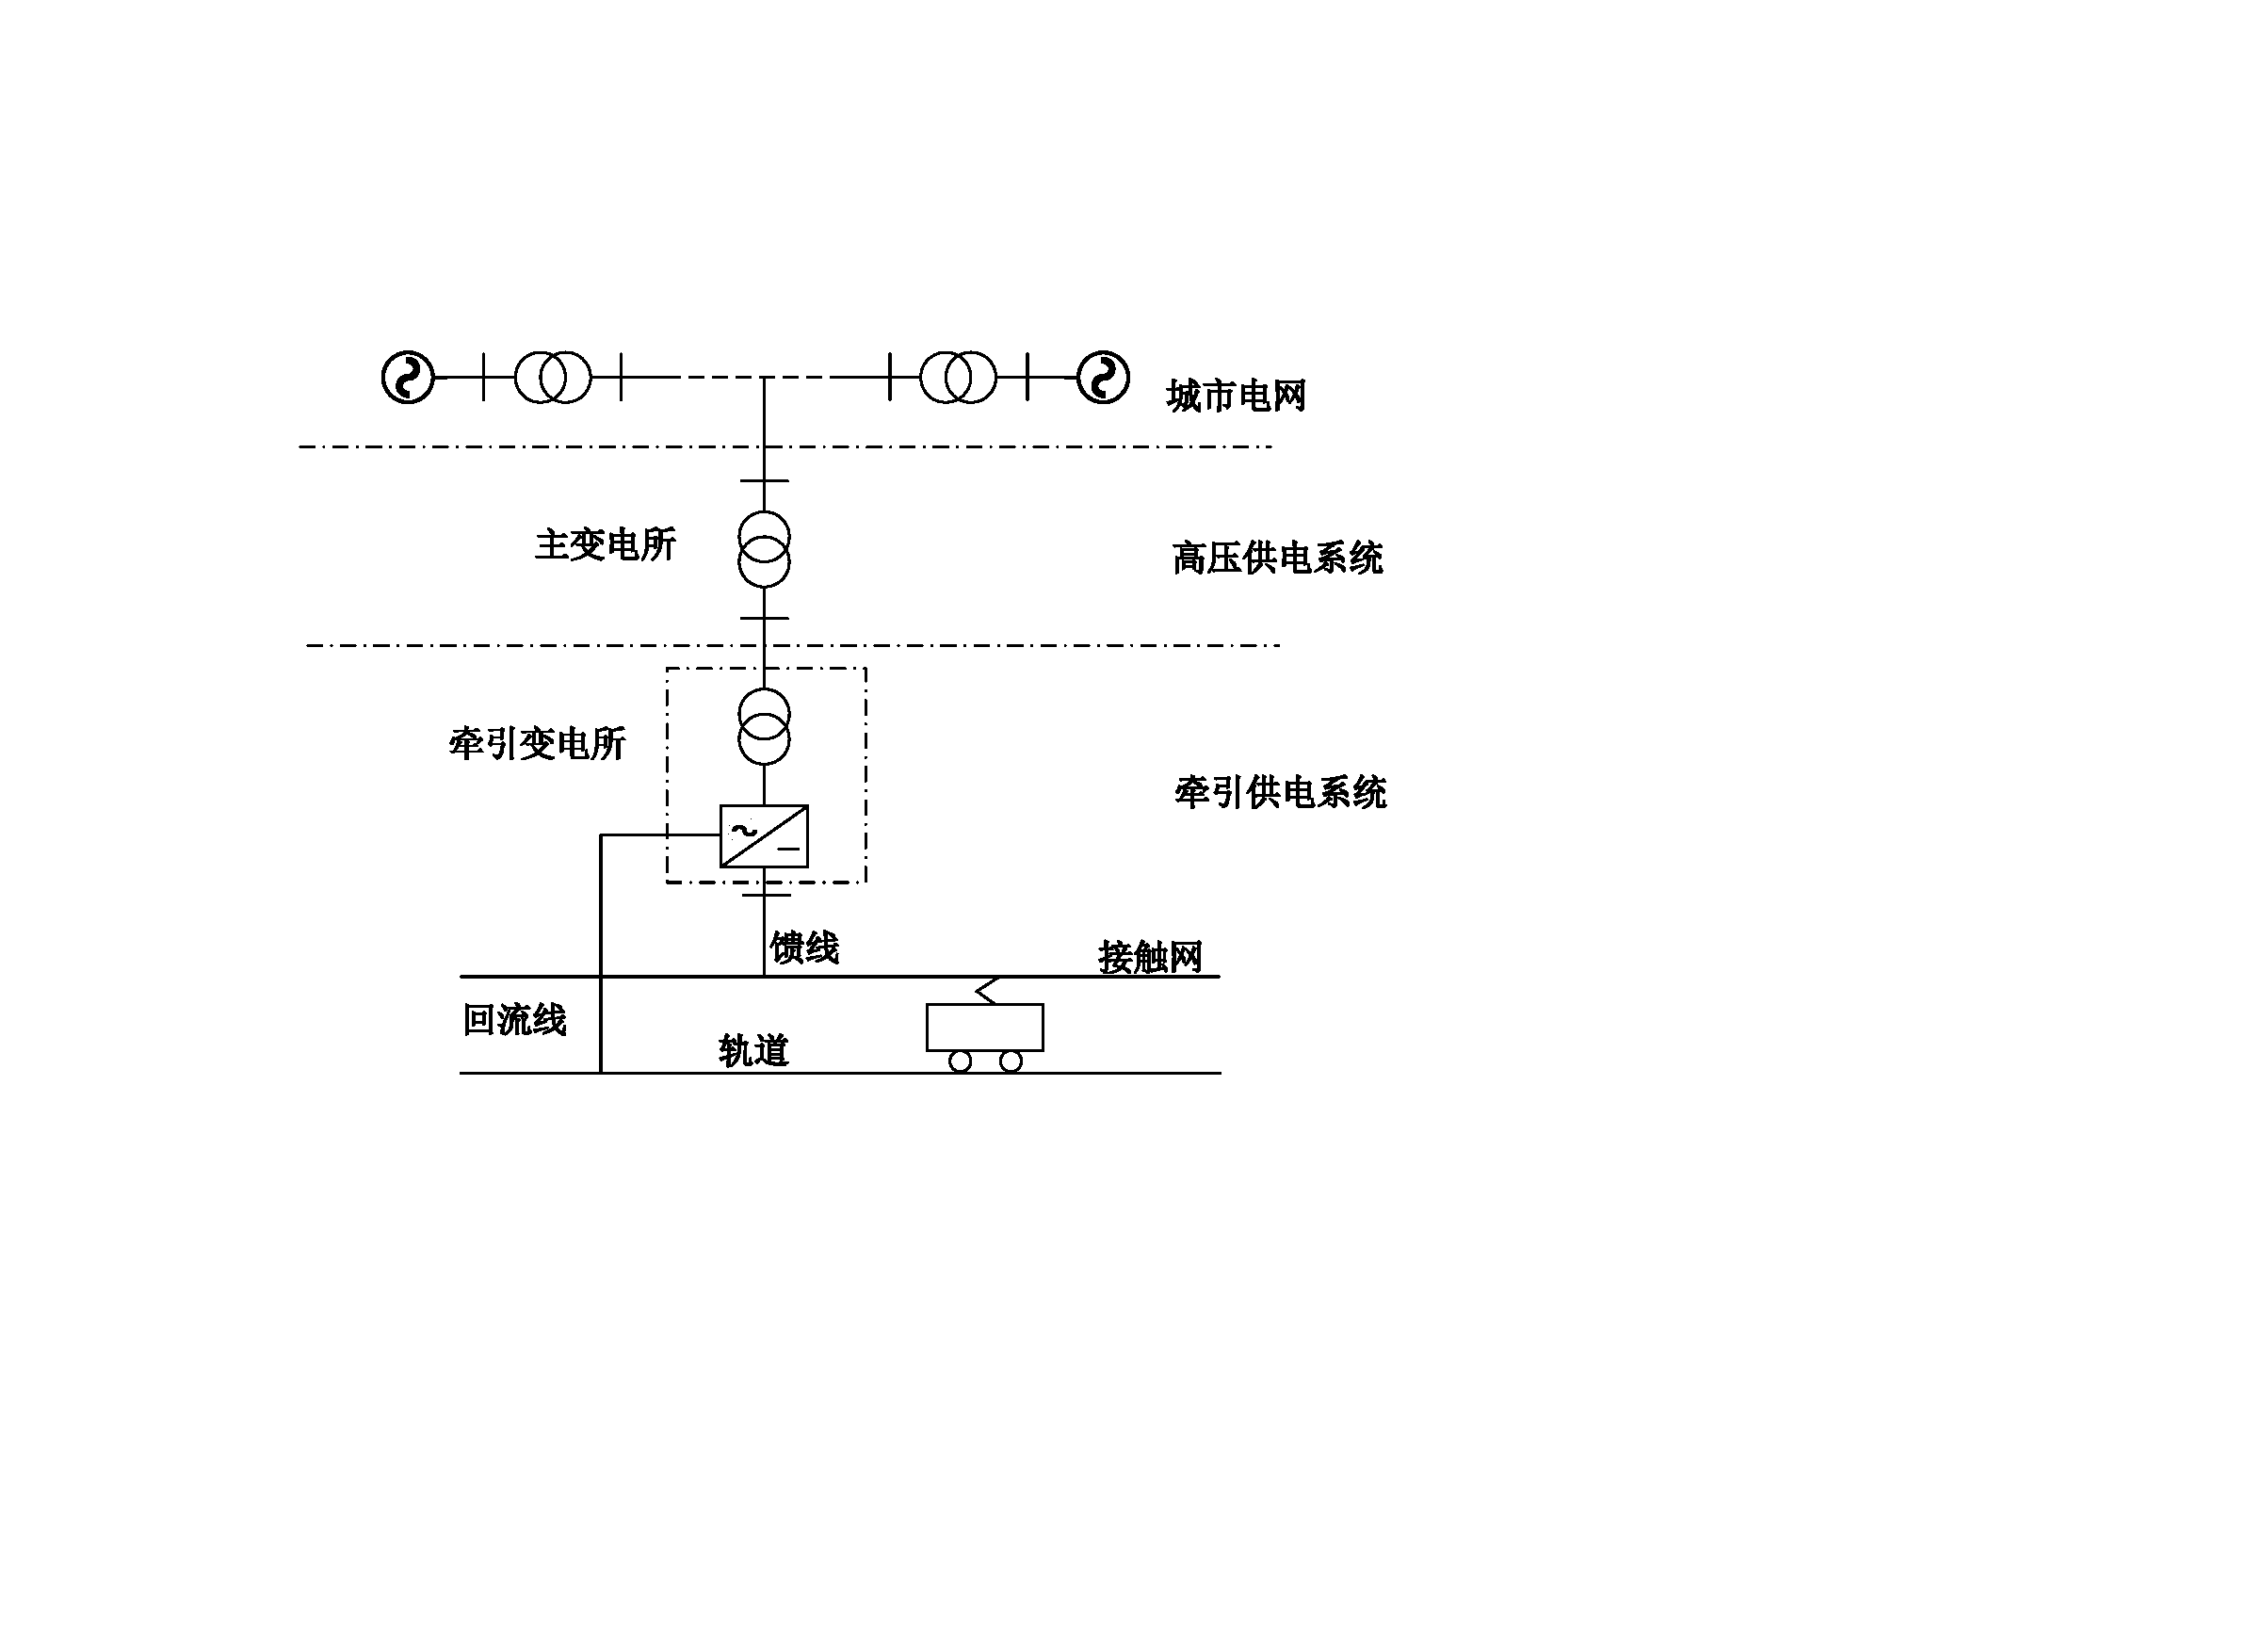
\includegraphics[width=0.7\linewidth]{figures/三级式供电}
	\caption{三级式供电}
	\label{fig:三级式供电}
\end{figure}

\section{主所数目}
地铁主变电所将城市电网的高压110KV(或220KV电能降压后以35KV或
10KV的电压等级分别供给牵引变电所和降压变电所。为保证供电的可靠性,
地铁线路通常设置两座或两座以上主变电所。
主变电所由两路独立的电源进线供电,内部设置2台相同的主变压器。
根据牵引负荷和动力负荷的不同情况,
主变压器可采用三相三绕组的有载调压变压器或双绕组的变压器。采用有
载调压变压器在电源进线电压波动时二次侧电压维持在正常值范围内。
主变电所为地铁线路的总变电所,承担整条地铁线路的电力负荷的用电。\newline
(1)可根据负荷计算确定在地铁线路上设置的主变电所数量。\newline
(2)每座主变电所设置2台主变压器,由城市电网地区变电站引入两路独立的
110KV专用线路供电,两回路同时运行,互为备用,以保证供电的可靠性和供电质量。
进线电源容量应满足远期时其供电区域内正常运行及故障运行情况下的供电要求。\newline
(3)低压35KV侧采用单母线分段接线,两段母线间设母联断路器,
正常运行时母联断路器打开。\newline
(4)正常运行时每座主变电所的两路110KV电源和2台主变压器分列运行。通过
35KV馈出电缆分别向各自供电区域的负荷和动力照明负荷供电。\newline
\section{牵引供电系统和动力照明系统采用何种方式}
通常,城市轨道交通动力照明配电方案总体可分为动力配电和照明配电。动力配电主要为车站各用电系统和用电设备提供电源,包括通风空调系统及设备,给排水系统及设备,FAS/BAS系统及设备,AFC、通信、外部通信、信号、公安通信等系统及设备,电梯、自动扶梯,安全门系统,卷帘门等;照明配电主要为车站照明、区间照明、场段照明等设备提供电源。所以在整个城市轨道交通项目建设全过程范围内,应在不同阶段对接口进行全面梳理并加强管理,才能保证系统运行的安全性、稳定性、系统性和可靠性。\par 
在满足计量、维修管理要求的情况下,应按照明负荷与动力负荷分开配电。一、二级负荷与三级负荷分开配电,车站与区间分开配电进行设计。通信系统、信号系统、火灾自动报警系统、电力监控系统、环境与设备监控系统、自动售检票系统等用电设备的配电应自成系统,由0.4kV低压开关柜室的一、二级负荷母线直接供电。排烟风机、送排风机、空调机、隧道风机等用电设备由通风空调电控柜供电,冷水机组由变电所供电。除环控设备外的其他动力设备及两端各半个区间动力设备均直接由降压变电所配电。\par 
为确保供电的稳定性,牵引供电系统和动力照明系统应该相互独立供电
\section{主接线形式分析}
方案Ⅰ:110kV采用内桥接线,35kV采用单母分段带旁路接线,10kV采用单母分段接线。\par 
\begin{figure}[!h]
	\centering
	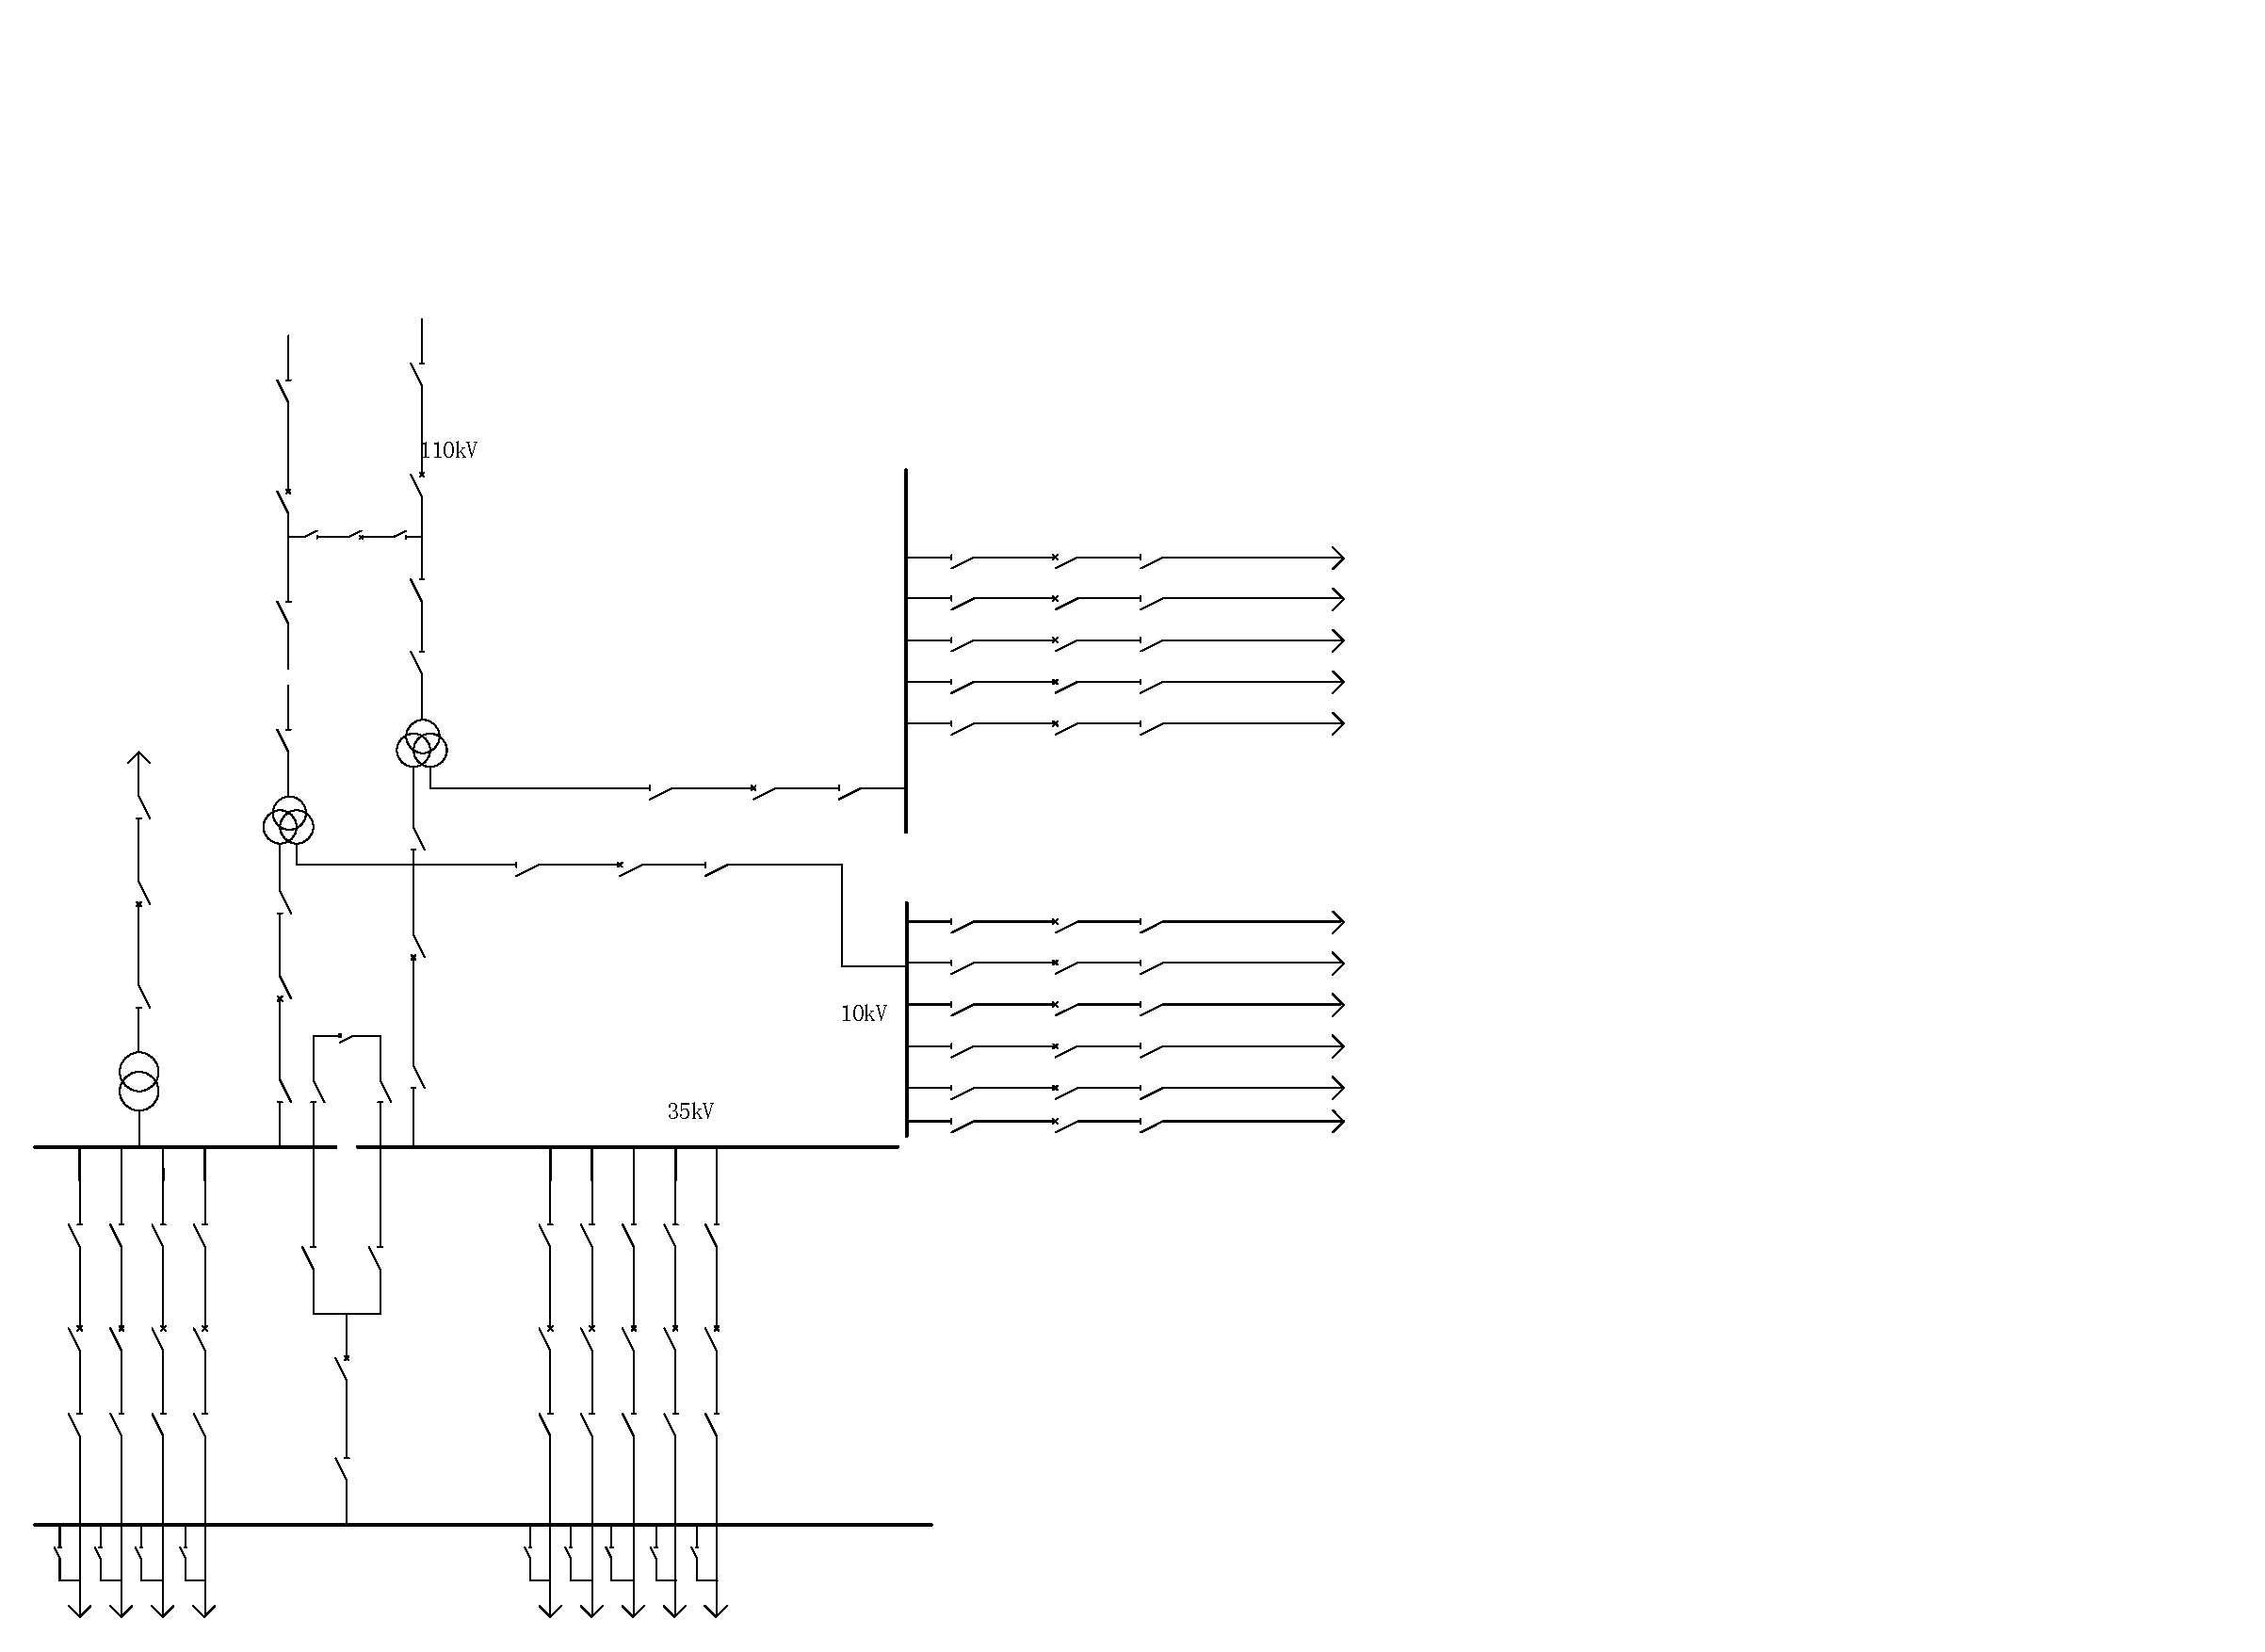
\includegraphics[width=0.5\textwidth]{方案I.pdf}
	\caption{方案I}
	\label{方案I}
\end{figure}
方案Ⅱ:110kV采用单母分段接线,35kV采用单母分段接线,10kV采用单母分段接线。\par 

\begin{figure}[!h]
	\centering
	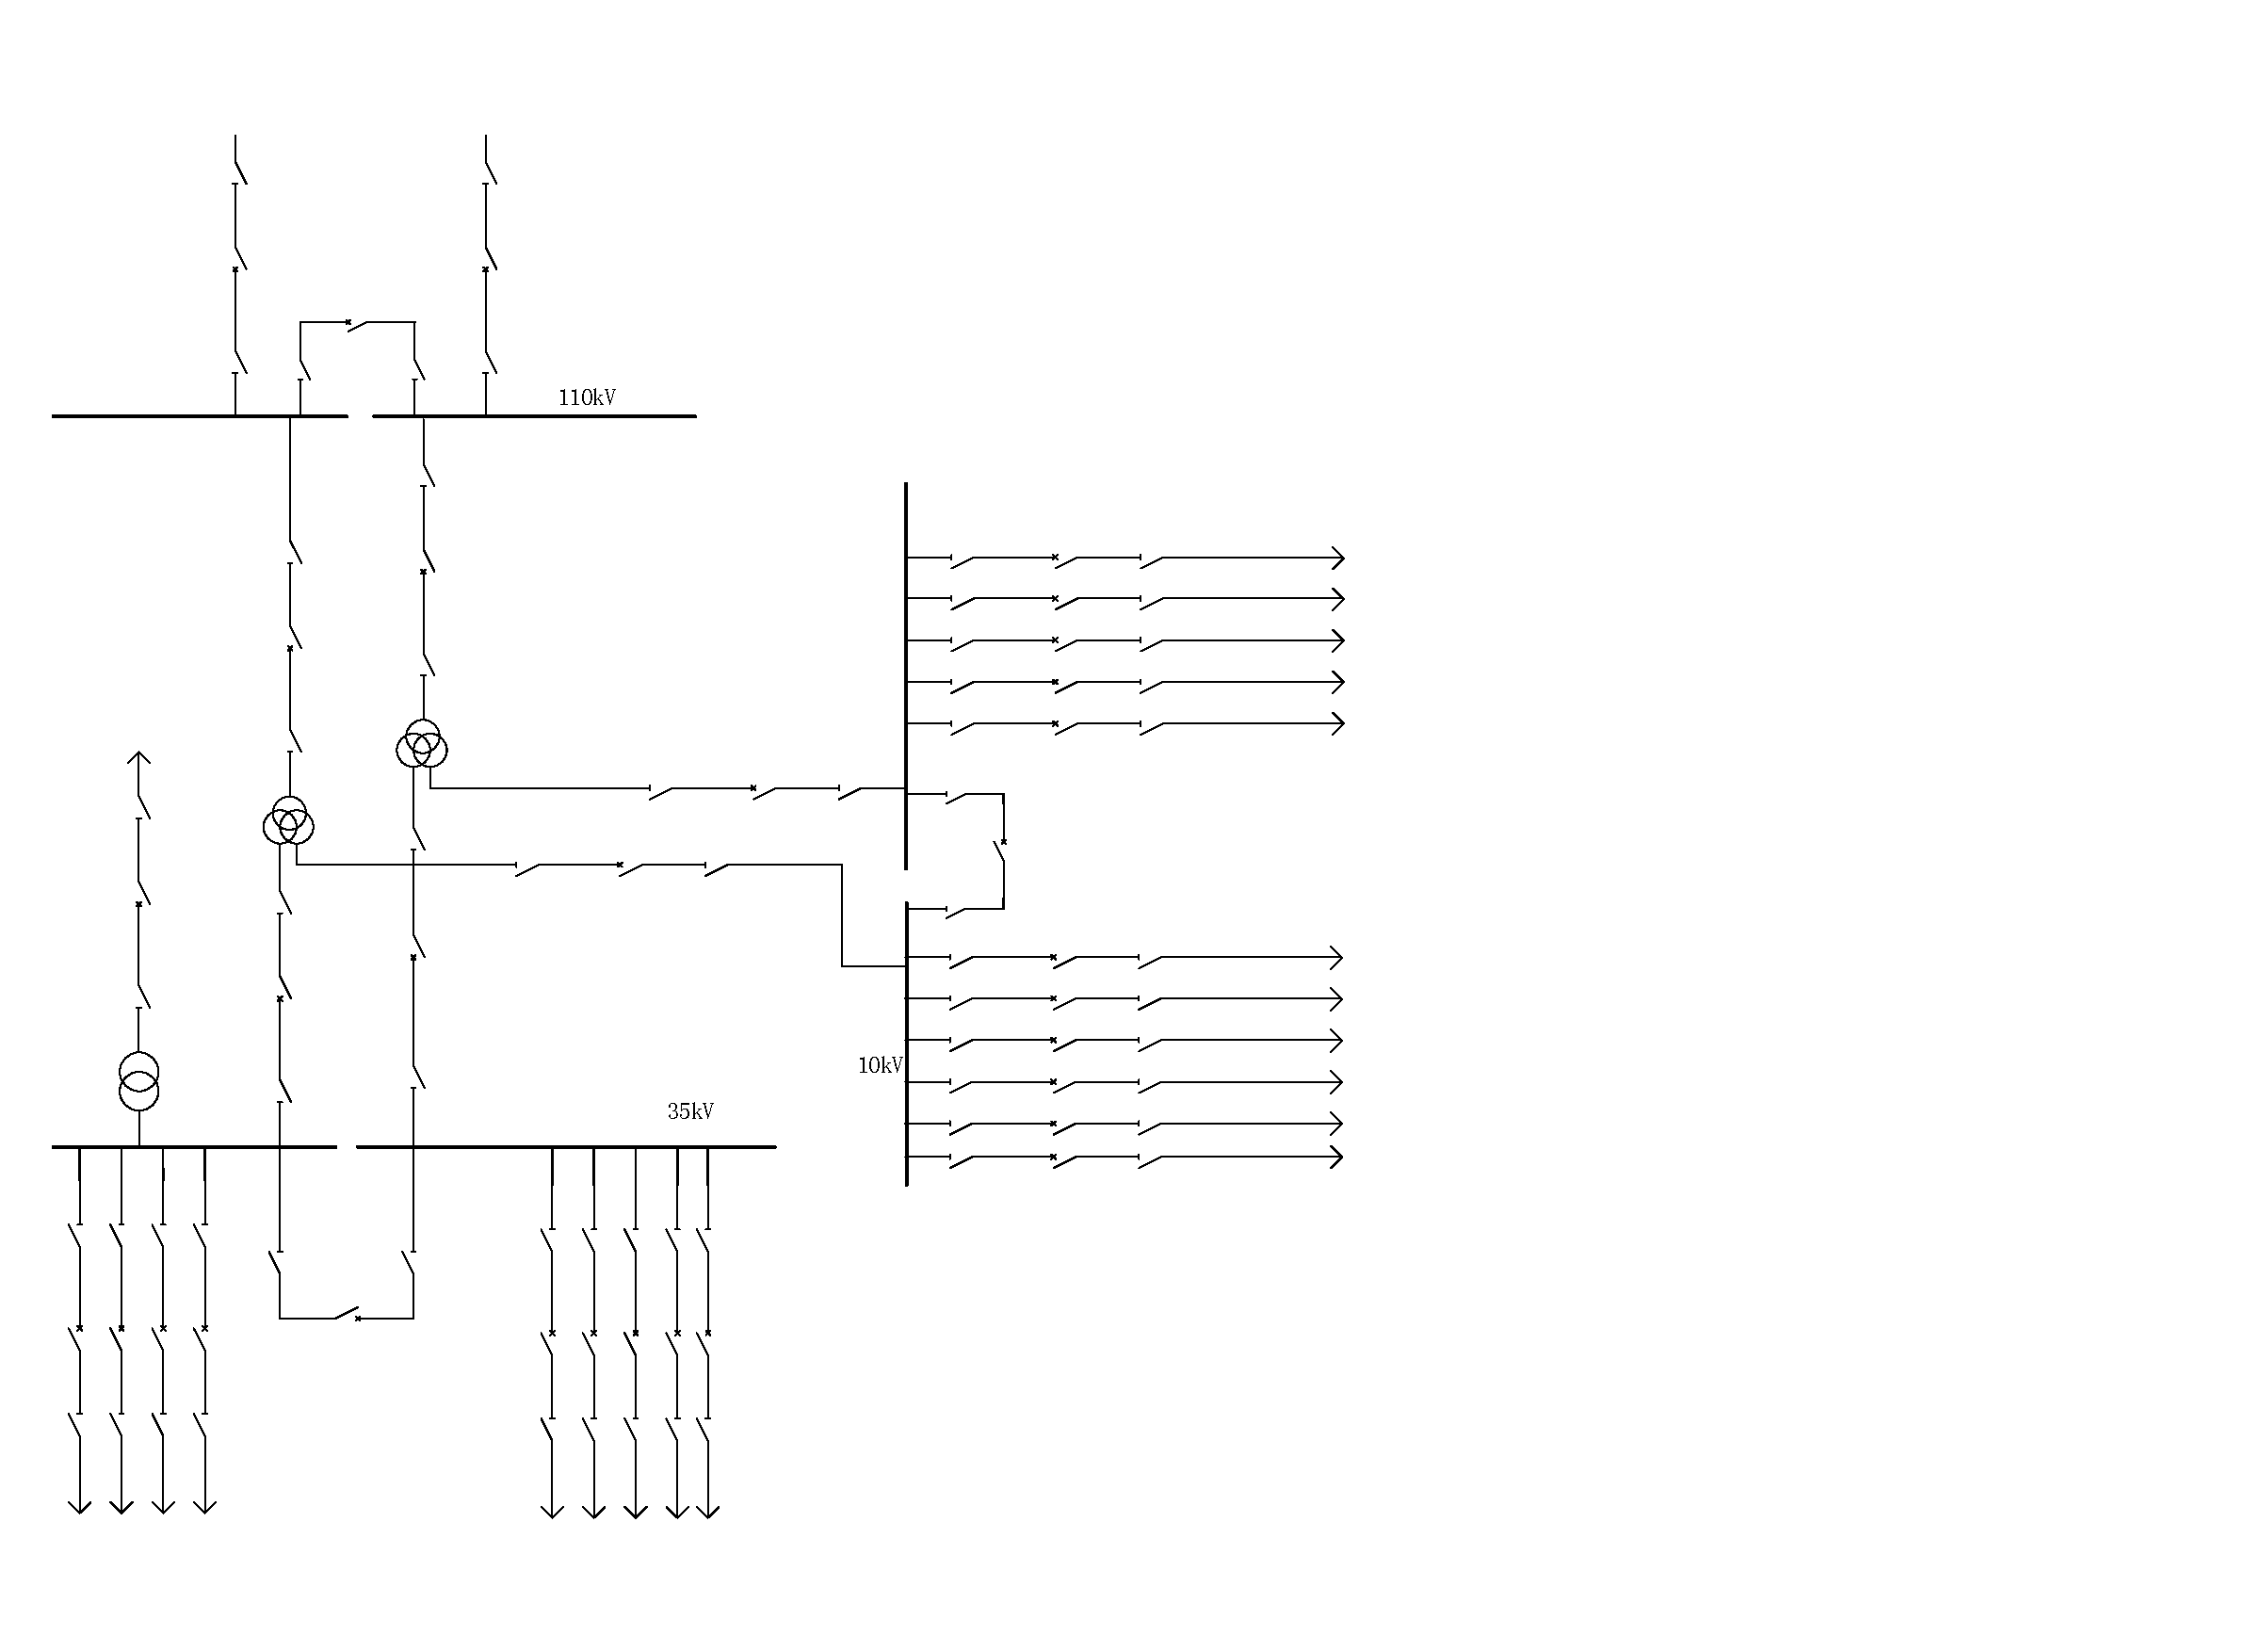
\includegraphics[width=0.5\textwidth]{方案II.pdf}
	\caption{方案II}
	\label{方案II}
\end{figure}
\subsection{主接线方案比较分析}
根据可靠性、灵活性、经济性对两种方案进行比较。\par 
(1)主接线方案的可靠性比较\newline
110kV侧:\newline
方案Ⅰ:采用内桥接线,当一条线路故障或切除、投入时,不影响变压器运行,不中断供电,并且操作简单;桥连断路器停运时,两回路将解列运行,亦不中断供电。且接线简单清晰,全部失电的可能性小,但变压器二次配电线及倒闸操作复杂,易出错。\newline
方案Ⅱ:采用单母线分段接线,任一台变压器或母线、线路故障或停运时,不影响其它回路的运行;分段断路器停运时,两段母线需解列运行,全部失电的可能稍小一些,不易误操作。\newline
35kA侧:\newline
方案Ⅰ:单母线分段兼旁路接线,检修任一台断路器时,都可用旁路断路器代替;当任一母线故障检修时,旁路断路器可代替该母线,使该母线的出线不致停运。\newline
方案Ⅱ:单母线分段接线,检修任一台断路器时,该回路需停运,分段开关停运时,两段母线需解列运行,当一段母线发生故障,分段断路器自动将故障段切除,保证正常段母线不至失电,另一段母线上其他线路需停运。\par 
(2)主接线方案的灵活性比较\newline
110kV侧:\newline
方案Ⅰ:操作时,主变压器的切除和投入较复杂,需动作两台断路器,扩建方便。线路的投入和切除比较方便。\newline
方案Ⅱ:调度操作时可以灵活地投入和切除线路及变压器,而且便于扩建。\newline
35kV侧:\newline
方案Ⅰ:运行方式较复杂,调度操作复杂,但可以灵活地投入和切除变压器和线路,能满足在事故运行方式、检修方式及特殊运行方式下的调度要求,较易于扩建。\newline
方案Ⅱ:运行方式简便,调度操作简单灵活,易于扩建,但当断路器检修时线路要停运,影响供电。\par 
(3)主接线方案的经济型比较
\begin{table}[!ht]
	\centering
	\begin{tabular}{|c|c|c|c|c|c|}
		\hline
		~ & \makecell{主变压器\\(台)}  & \makecell{110kV\\断路器(台)}  & \makecell{110kV\\隔离开关(组)}  & \makecell{35kV\\断路器(台)}  & \makecell{35kV\\隔离开关(组)} \\ \hline
		Ⅰ & 2 & 3 & 8 & 13 & 35 \\ \hline
		Ⅱ & 2 & 5 & 10 & 12 & 33 \\ \hline
	\end{tabular}
	\caption{不同方案所需设备个数}
	\label{不同方案所需设备个数}
\end{table}\par 
从表\ref{不同方案所需设备个数}中可以看出,方案Ⅰ比方案Ⅱ综合投资少一些。\par 
(4)主接线方案的确定\newline
对方案Ⅰ、方案Ⅱ进行综合比较,根据它们的可靠性、灵活性和经济性,最终选择了方案一。 

\subsection{主变压器接线形式}
在330kV及以下的变电站中,一般都选用三相式变压器。因为一台三相式变压器较同容量的三台单相式变压器投资小、占地少、损耗小,同时配电装置结构较简单,运行维护较方便。在有三种电压等级的变电站中,如果变压器各侧绕组的通过容量均达到变压器额定容量的15\%及以上,或低压侧虽然无负荷,但需要在该侧装无功补偿设备时,宜采用三绕组变压器。我国110kV及以上电压,变压器绕组都采用星形接法,35kV也采用星形接法,其中性点多通过消弧线圈接地。35KV及以下电压,变压器绕组都采用三角形接法。
\section{牵降混合所主接线分析}

\subsection{35KV交流侧牵引降压混合所主接线}
目前常见的接线方式多为以下几类:双母线接线、单母线接线、单母线带旁路母线接线、单母分段接线。\par 
考虑到典型牵引降压混合变电所的主接线对于可靠性、灵活性要求较高,且要考虑一定的经济性,我们选用单母线分段接线作为35kV交流测的主接线。\par 
单母线分段接线具有供电可靠性高的优点。当一段母线发生故障,分段断路器自动将故障段切除,保证正常母线不间断供电和不致使重要用户停电。且用断路器将母线分段后,对重要负荷可以从不同段引出两回路,提供双回路供电。调度灵活性高,变压器投切比较方便。当任意电源故障或检修时,可由母联开关替代,避免母线停电。\par 
但值得注意的是,当出线或出线断路器、隔离关故障或检修时,该回路将停止供电。扩建时需要向两个方向均衡扩建,以保证负荷分配的均匀。当出线回路为双回路时,常使母线出线交叉跨越。\par 
单母分段接线\par 
\begin{figure}[!h]
	\centering
	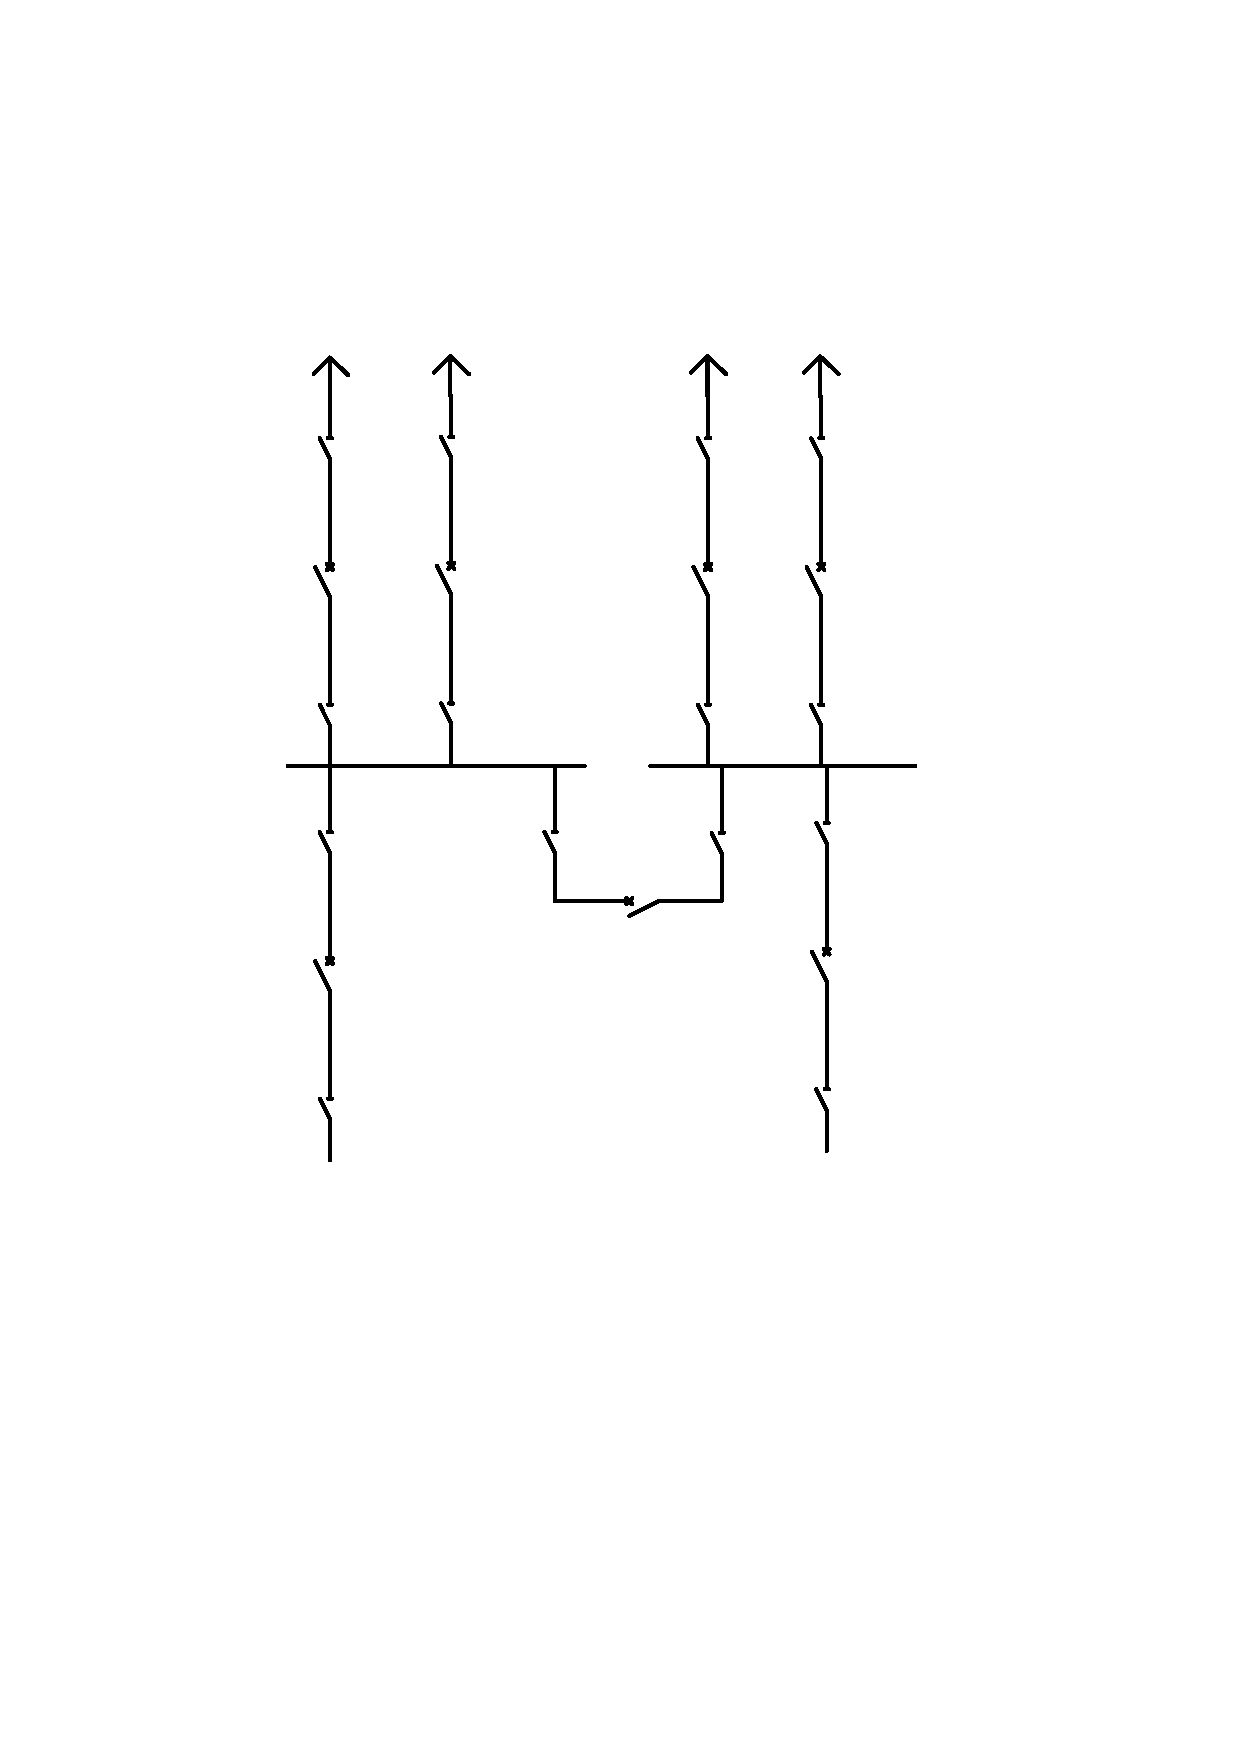
\includegraphics[width=0.5\textwidth]{单母线分段.pdf}
	\caption{单母线分段接线}
	\label{单母线分段接线}
\end{figure}
优点:供电可靠性高。当一段母线发生故障,分段断路器自动将故障段切除,保证正常母线不间断供电和不致使重要用户停电。且用断路器将母线分段后,对重要负荷可以从不同段引出两回路,提供双回路供电。调度灵活性高,变压器投切比较方便。当任意电源故障或检修时,可由母联开关替代,避免母线停电。\par
缺点:当出线或出线断路器、隔离关故障或检修时,该回路将停止供电。扩建时需要向两个方向均衡扩建,以保证负荷分配的均匀。当出线回路为双回路时,常使母线出线交叉跨越。\par
考虑到该变电所要求供电可靠性比较高,并且出于经济成本考虑,所以最终决定选用单母线分段的主接线方式作为35KV交流侧的主接线方式。
\subsection{1500V直流侧牵引降压混合所主接线}
根据城轨交通牵引负荷的特点和国内外运营经验, 其牵引变电所主接线的直流部分, 一般采用单母线接线的形式。\par 

\begin{figure}[h]
	\centering
	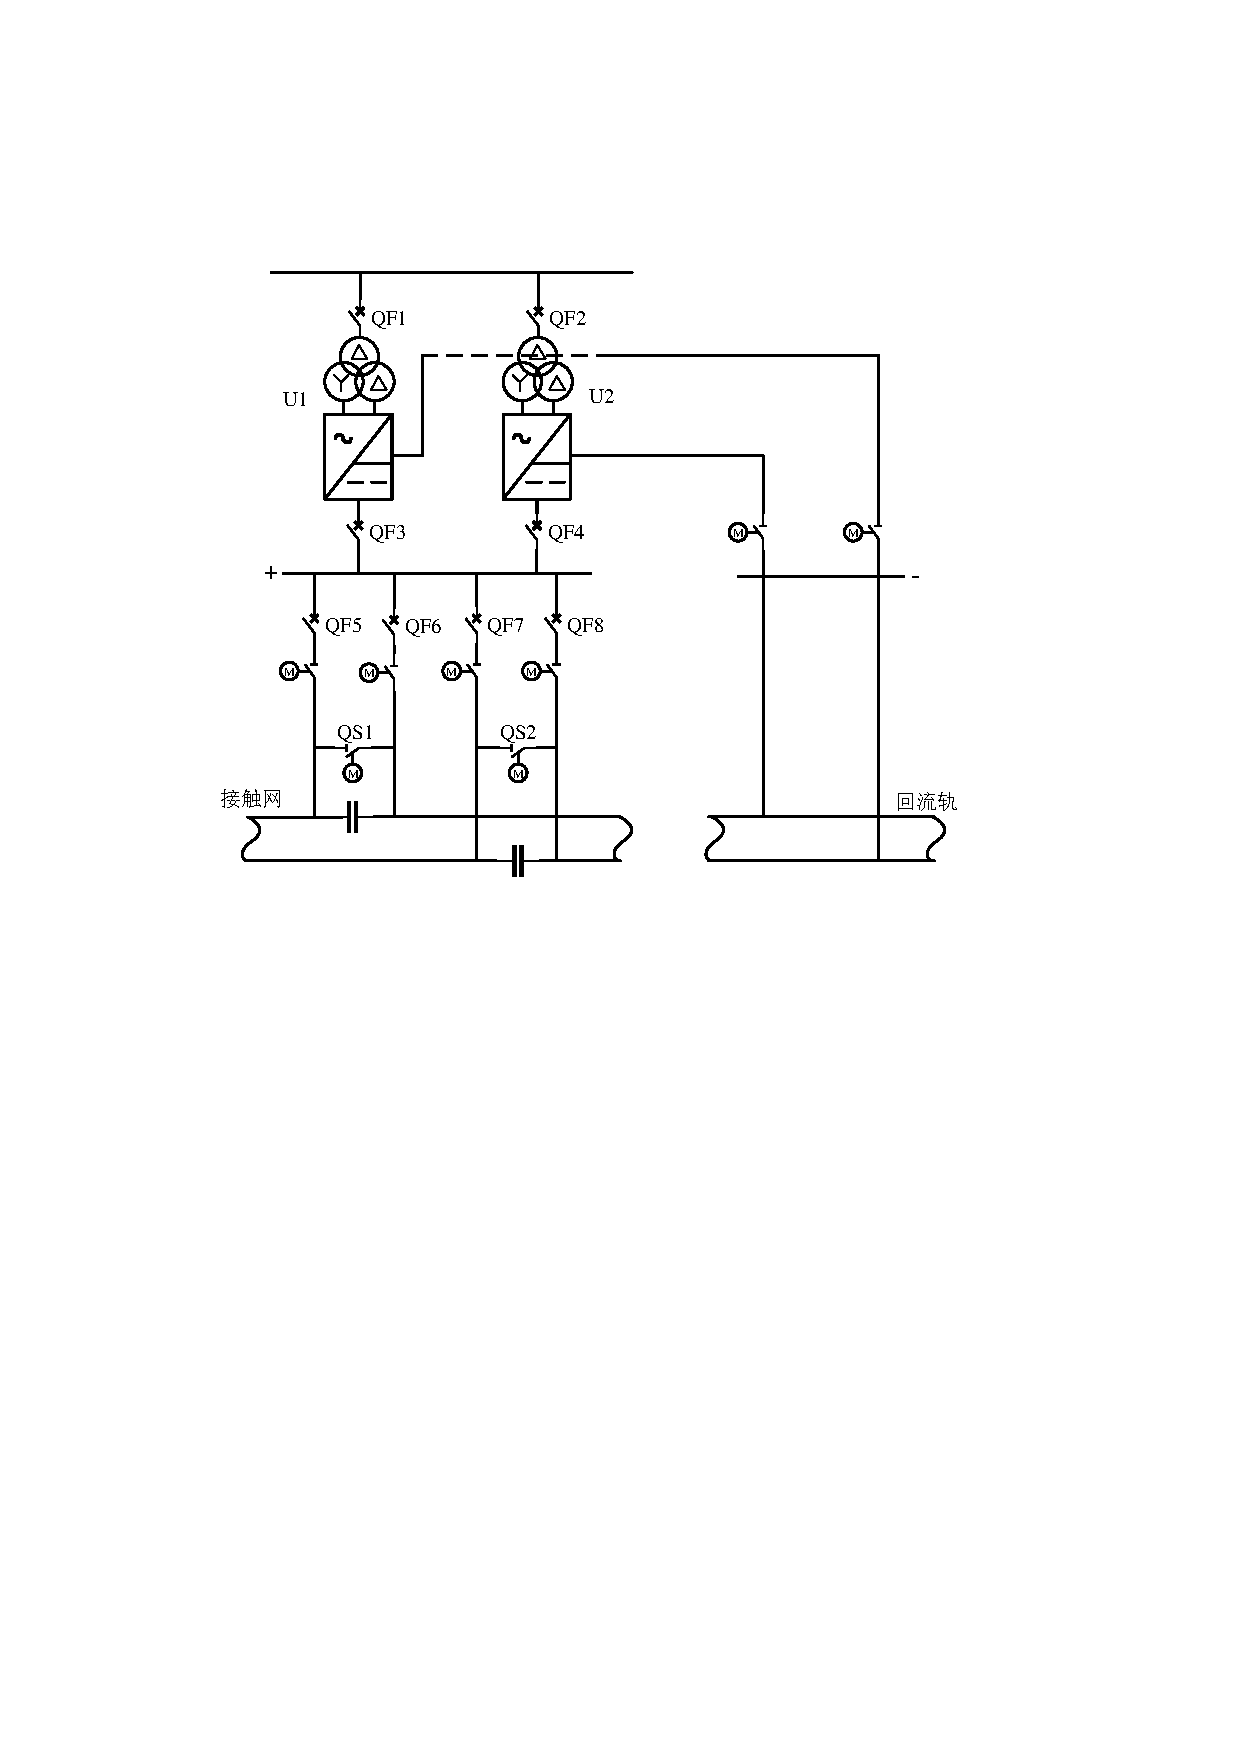
\includegraphics[width=0.5\textwidth]{牵引所主接线.pdf}
	\caption{牵引所主接线}
	\label{牵引所主接线}
\end{figure}
直流主接线应重视国内外长期运行的实践经验及可靠性的定性分析。可靠性的衡量标准是运行实践。可靠性的定量分析由于数据及计算方法尚不完善, 计算结果不够准确, 因而目前仅作为参考。该方式是最早被用于城轨交通牵引变电所直流母线的接线方式之一,用于我国20世纪60年代中期建造的第一条城轨交通线——北京地铁一号线。由于当时采用的是前苏联的固定式直流设备,所以采用此种直流主接线方式,应该说是比较好的选择。该方式在前苏联及东欧一些国家的城轨交通的牵引供电中得到广泛的应用,实践证明其运行可靠。\par 
运行方式分析:\par 
(1)正常状态。在正常状态下,可通过直流断路器向牵引网提供直流电源。\par 
(2)事故状态。事故状态分为断路器故障、牵引网或直流电缆故障、接地故障。 \par
a.在断路器故障时,采用该方式可通过倒闸作业,退出故障断路器,并投入备用断路器。使用该方式,检修人员可用备用断路器小车替换故障断路器。\par
b.牵引网或直流电缆故障。在直流电缆故障时,可使相应馈线的断路器跳闸,通过牵引网越区隔离开关的倒闸作业,由相邻的馈线回路向停电的牵引网提供电源;在牵引网过负荷或短路故障时,可通过相应馈线的断路器经过判断后跳闸,使故障段退出运行。\par
c.接地故障。当直流设备发生碰壳故障时(变电所所有直流设备),框架保护装置启动,故障变电所退出运行,由临近变电所实现双边(或单边)供电。
\section{降压所主接线}
    供电方式问题:\par 

牵引供电系统设计时考虑了双边供电,但单边供电是一种仅在必要情况下采用的临时供电方式,不是制约牵引供电规划的条件。双边供电是城市轨道交通最基本的供电方式,是设计的首要选择,也是运营的首选方案。\par 

\subsection{中压主接线和运行方式}

(1) 中压主接线采用单母线分段接线:在牵引系统的中压一侧,我们采用单母线分段的方式,并配置了分段开关。在正常运行时,两个独立的电源同时供电,两段母线并行运行。\par 

(2) 运行方式:\par
a. 正常运行:在正常情况下,两个独立电源同时供电,两段母线并行运行。\par
b. 进线电源失效运行:如果其中一个进线电源失效,分段开关会自动切换,使另一个进线电源向本牵引变电所的两段母线供电。当两个进线电源都失效时,通过调度进行倒闸操作,从相邻变电所获取中压电源。\par
c. 母线故障运行:如果某一段母线发生故障,分段开关将保持关闭,不切换到运行状态。另一段母线将继续供电。在这种情况下,如果有牵引整流机组连接到故障的母线上,它将停止运行,而直流牵引系统将通过内部操作实施大规模的双边供电。当两段母线都出现问题时,本牵引站将停止运行。
\begin{figure}[!h]
	\centering
	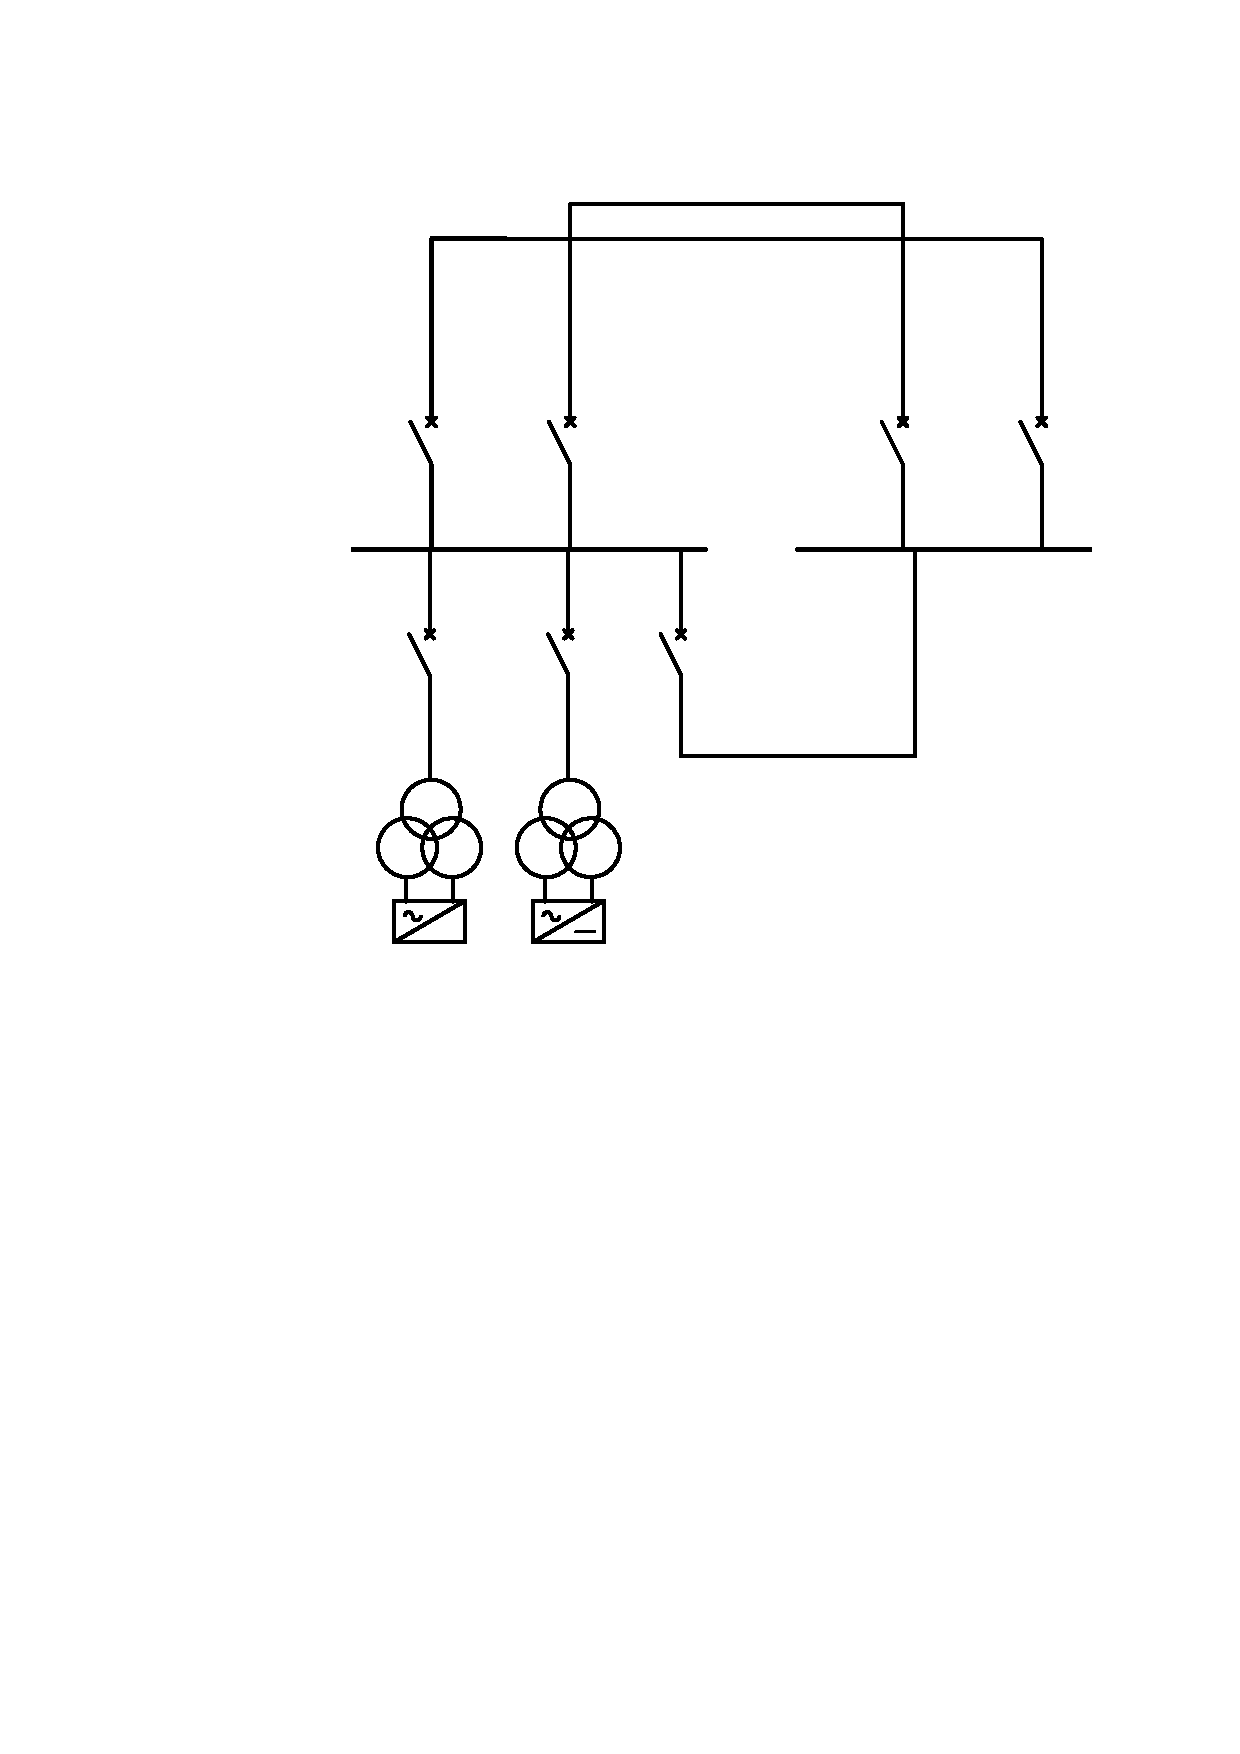
\includegraphics[width=0.7\textwidth]{分段单母线.pdf}
	\caption{分段单母线}
	
\end{figure}

\subsection{直流主接线和运行方式}

(1) 采用A型单母线系统的直流主接线:我们使用两路进线,配备直流断路器,并设置了四路直流馈出线。牵引整流机组的负极使用电动隔离开关。在同一馈电区分段的上下行之间,设有纵向电动隔离开关。\par 

(2) 运行方式:\par 
a. 正常运行:在正常运行时,采用24脉波整流,两台整流机组并列运行。直流进线开关、馈线开关、上网电动隔离开关都处于闭合状态,纵向电动隔离开关处于断开状态。此变电所与相邻变电所对同一供电区域实施正常的双边供电。\par 
b. 单台整流机组停机:如果整流机组R1发生故障,进线开关1041跳闸,201联动跳闸。馈线开关和上网电动隔离开关都处于闭合状态,纵向电动隔离开关处于断开状态。这时采用12脉波正常双边供电。\par 
c. 两台整流机组停机:如果整流机组R1和R2都故障停机,进线开关1041和1042跳闸,201和202联动跳闸。控制中心会对上报的保护信息进行判断,如果不是直流母线短路或框架保护触发,那么211、212、213、214将被合上,纵向中压隔离开关2113和2124将被断开。\par 
d. 直流母线停机:为应对开关柜直流母线碰壳故障,我们设置了框架泄漏电流保护。当开关柜直流母线发生故障时,框架保护会联动切断所有馈线开关、两台整流机组进线开关以及上下行相邻牵引站的相应馈出开关(这些相邻站的开关可以由人工合闸)。控制中心将远程分闸上网隔离开关,合上纵向电动隔离开关2113和2124,通过纵向隔离开关实施大规模的双进供电。\par 
e. 单台馈线开关停机:当单台馈线开关211停机时,211和其对应的上网电动隔离开关都会断开,相关的纵向电动隔离开关2113将被合上。\par 
f. 分段运行两侧上(下)行的两台馈线开关停机:当上行的211和213停机时,相关的上网隔离开关将被分闸,远程合上纵向电动隔离开关2113(满足合闸条件),从而实现大规模双边供电。下行的212、214及其相关上网隔离开关将保持合闸状态,2124将被分闸,以维持正常的双边供电状态。
\begin{figure}[!h]
	\centering
	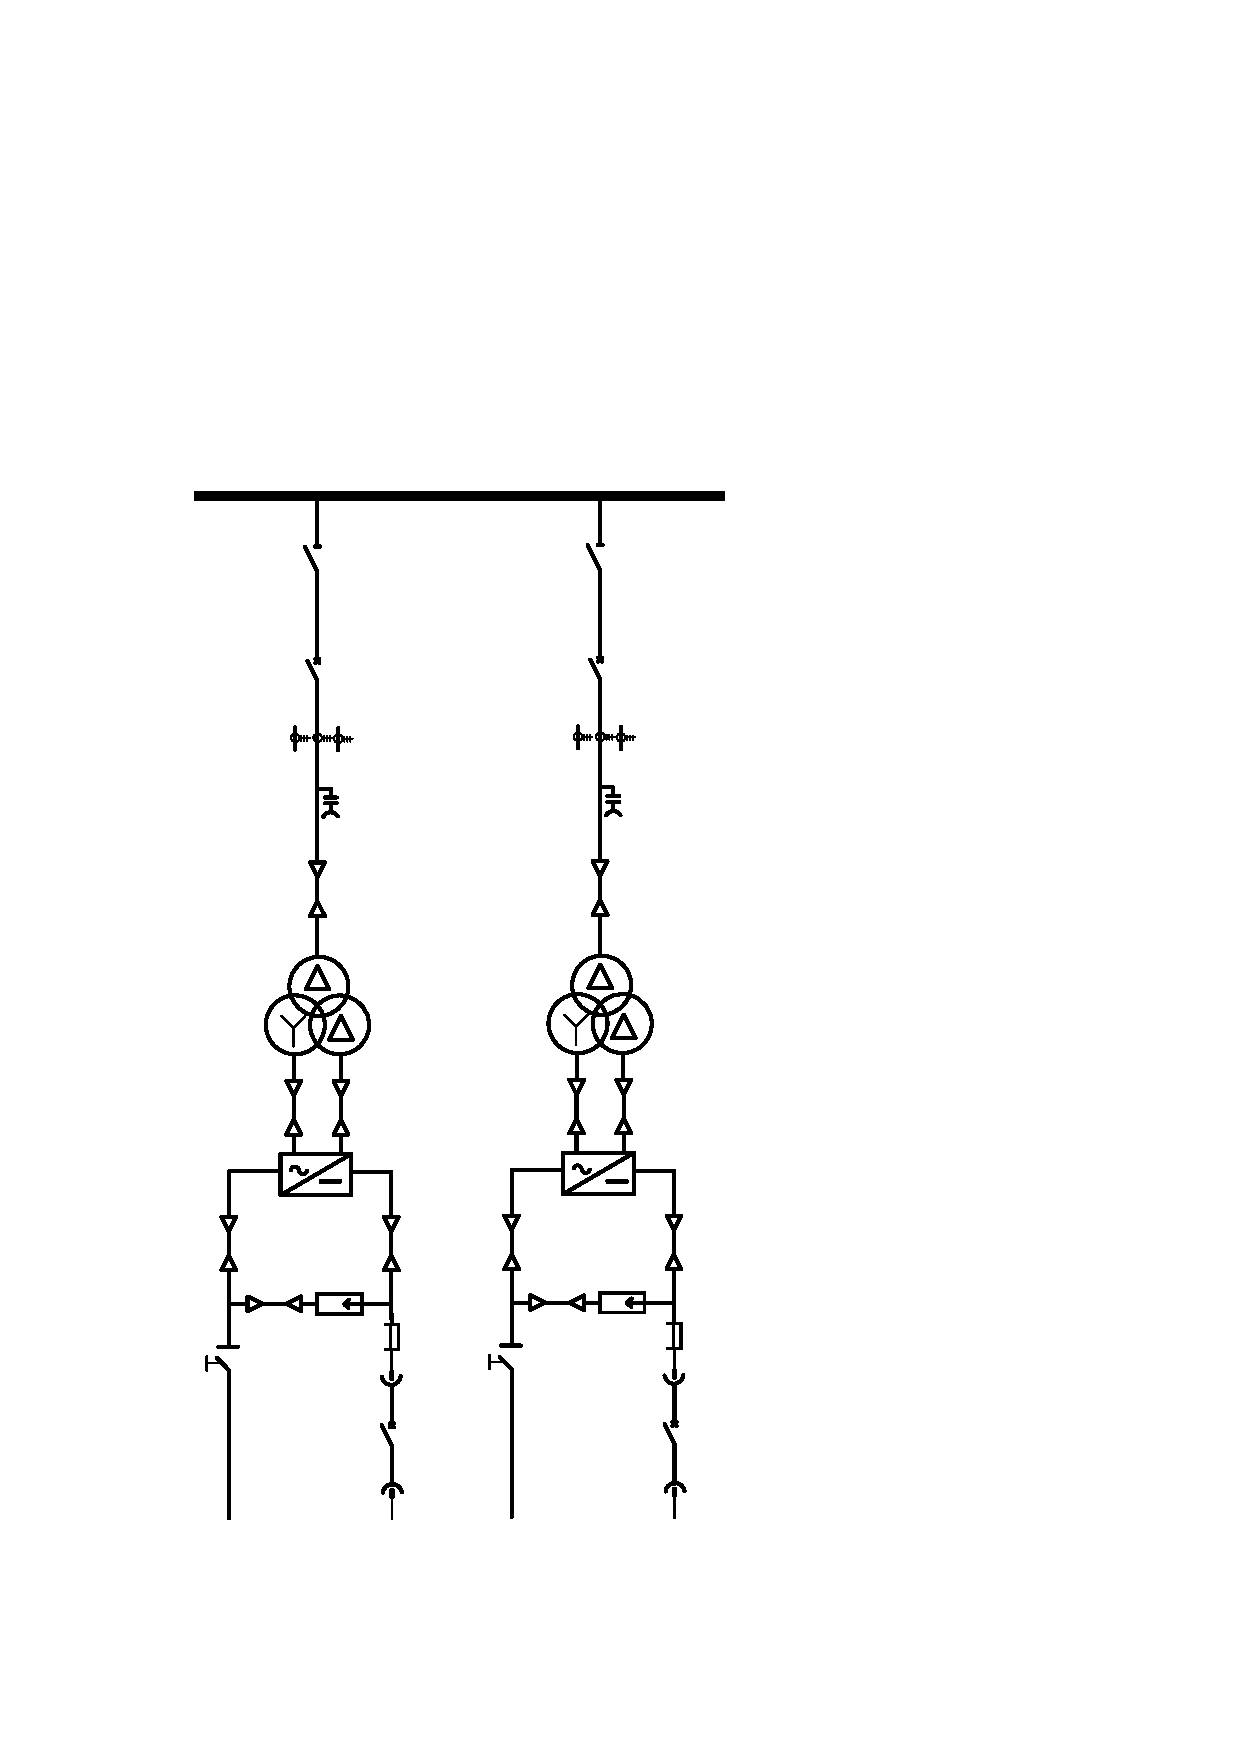
\includegraphics[width=0.5\textwidth]{直流主接线.pdf}
	\caption{直流主接线}
	\label{直流主接线}
\end{figure}
\subsection{降压部分}
1. 不同负荷供电要求:\par 

一级负荷需要双路电源供电,这两路电源分别来自降压变电所的两个独立母线段,实现自动切换在负载端。\par 
二级负荷的电源可以从降压变电所的任一母线段获得。当其中一路电源失效时,母联开关可以手动或自动切换至备用电源。\par 
三级负荷通过分配箱引出单一电源供电,允许随时进行切除。\par 

2. 主接线形式:\par 

中压母线采用单母线分段的形式,并配置联络开关。\par 
我们设置了两个独立的进线和两个出线,以确保可靠供电。\par 
两个配电变压器各自连接到中压母线的一个段。\par 
0.4KV母线也采用单母线分段,同样配备联络开关。
\addtocounter{page}{-1}